%%%%%%%%%%%%%%%%%%%%%%%%%%%%%%%%%%%%%%%%%%%%%%%%%%%%%%%%%%%%%%%%%%%%%%%%%%%%%%%%%%
\begin{frame}[fragile]\frametitle{}
\begin{center}
{\Large Generative AI}
\end{center}
\end{frame}

%%%%%%%%%%%%%%%%%%%%%%%%%%%%%%%%%%%%%%%%%%%%%%%%%%%%%%%%%%%%%%%%%%%%%%%%%%%%%%%%%%
\section{Introduction}

%%%%%%%%%%%%%%%%%%%%%%%%%%%%%%%%%%%%%%%%%%%%%%%%%%%%%%%%%%%%%%%%%%%%%%%%%%%%%%%%%%
\begin{frame}[fragile]{Introduction}
\begin{itemize}
\item Generative AI rapidly generates new data using machine learning algorithms.
\item Google is a leading company in generative AI, offering tools and frameworks.
\item This presentation covers concepts, framework, applications, and conclusion of Google's generative AI.
\end{itemize}
\end{frame}

%%%%%%%%%%%%%%%%%%%%%%%%%%%%%%%%%%%%%%%%%%%%%%%%%%%%%%%%%%%%%%%%%%%%%%%%%%%%%%%%%%
\begin{frame}[fragile]{Difference}
Lets see how the solutions to the problem of detecting a cat from images using traditional programming, deep learning, and generative AI, respectively.
\end{frame}

%%%%%%%%%%%%%%%%%%%%%%%%%%%%%%%%%%%%%%%%%%%%%%%%%%%%%%%%%%%%%%%%%%%%%%%%%%%%%%%%%%
\begin{frame}[fragile]{Traditional Programming}
  \begin{itemize}
    \item Traditional programming involves writing explicit rules to detect a cat in images.
    \item Features like color, texture, and shape can be used to define these rules.
    \item However, designing accurate rules for complex patterns like cat detection can be challenging.
    \item It requires extensive domain knowledge and might not generalize well to different images.
  \end{itemize}
  
\begin{center}
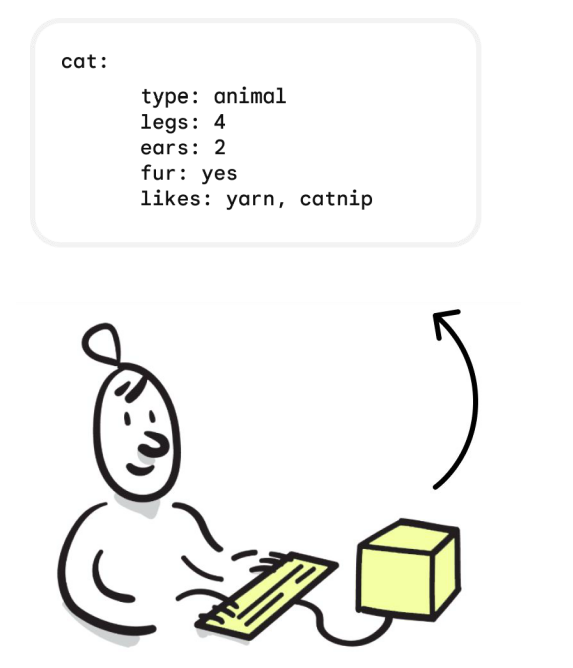
\includegraphics[width=0.3\linewidth,keepaspectratio]{genai1}
\end{center}

{\tiny (Ref: Primer on LLM and Gen AI - Google Cloud)}
  
\end{frame}

%%%%%%%%%%%%%%%%%%%%%%%%%%%%%%%%%%%%%%%%%%%%%%%%%%%%%%%%%%%%%%%%%%%%%%%%%%%%%%%%%%
\begin{frame}[fragile]{Deep Learning}
  \begin{itemize}
    \item Deep learning utilizes neural networks to automatically learn features for cat detection.
    \item Convolutional Neural Networks (CNNs) are particularly effective for image classification tasks.
    \item Large labeled datasets of cat images are used to train the network.
    \item The network learns to identify unique cat features and generalize them to detect cats in new images.
    \item Deep learning offers better accuracy and can handle complex patterns without explicit rule definition.
  \end{itemize}
  
\begin{center}
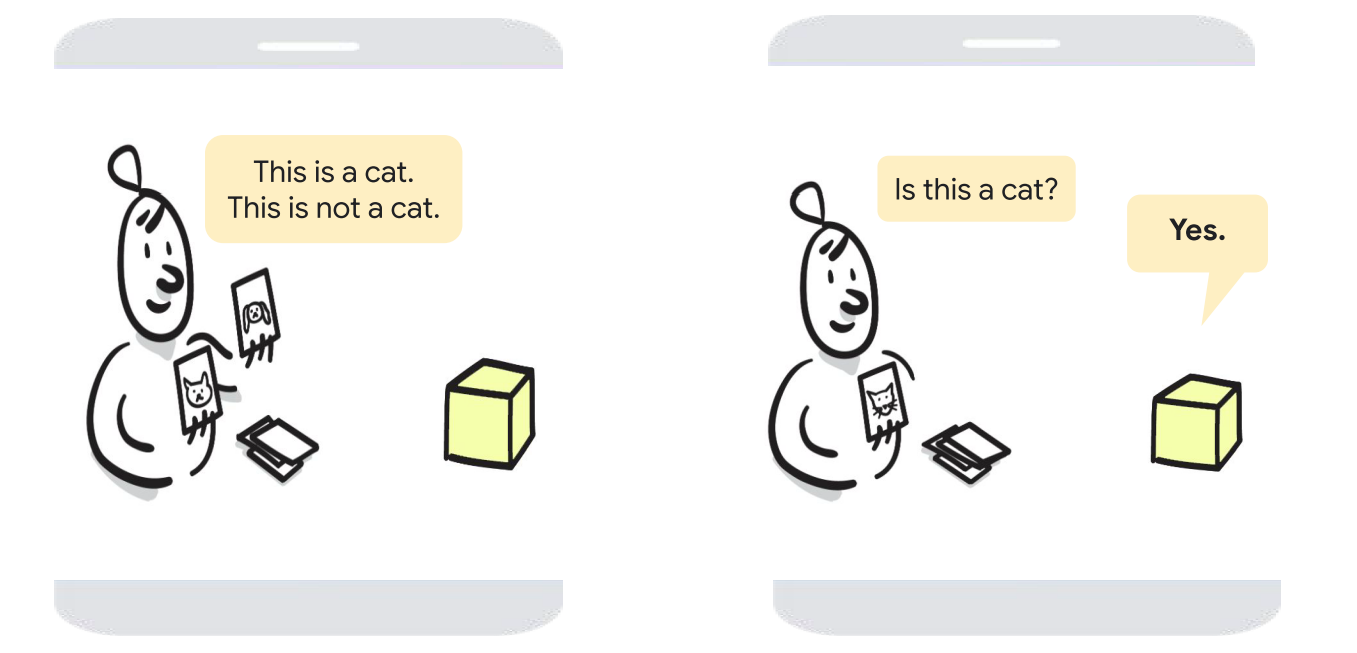
\includegraphics[width=0.4\linewidth,keepaspectratio]{genai2}
\end{center}

{\tiny (Ref: Primer on LLM and Gen AI - Google Cloud)}  
\end{frame}

%%%%%%%%%%%%%%%%%%%%%%%%%%%%%%%%%%%%%%%%%%%%%%%%%%%%%%%%%%%%%%%%%%%%%%%%%%%%%%%%%%
\begin{frame}[fragile]{Generative AI}
  \begin{itemize}
    \item Generative AI focuses on generating new data, including images of cats.
    \item Generative Adversarial Networks (GANs) are used to generate realistic cat images.
    \item The GAN consists of a generator and a discriminator that compete against each other.
    \item The generator learns to generate increasingly realistic cat images, while the discriminator learns to distinguish real from generated images.
    \item The generated cat images can be used to augment datasets for cat detection models.
  \end{itemize}
  
\begin{center}
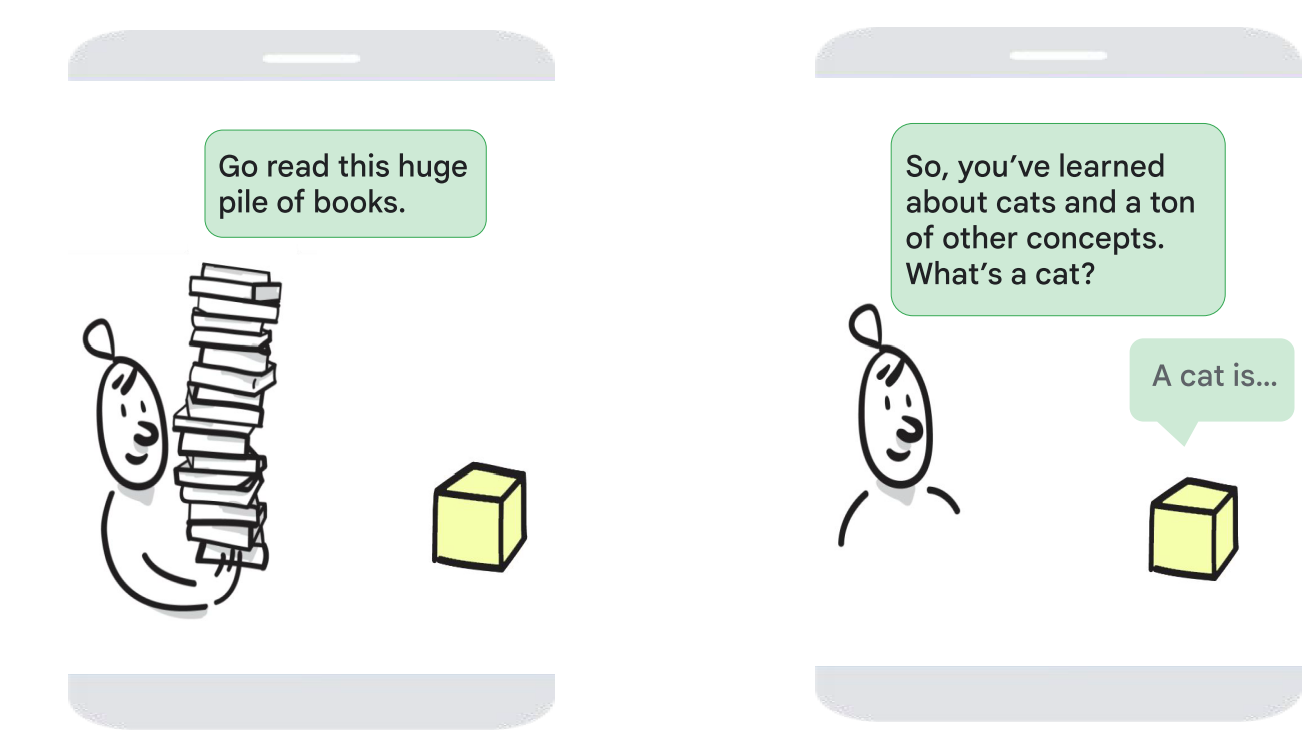
\includegraphics[width=0.5\linewidth,keepaspectratio]{genai3}
\end{center}

{\tiny (Ref: Primer on LLM and Gen AI - Google Cloud)}
  
\end{frame}

%%%%%%%%%%%%%%%%%%%%%%%%%%%%%%%%%%%%%%%%%%%%%%%%%%%%%%%%%%%%%%%%%%%%%%%%%%%%%%%%%%
\begin{frame}[fragile]{The Start \ldots}

\begin{center}
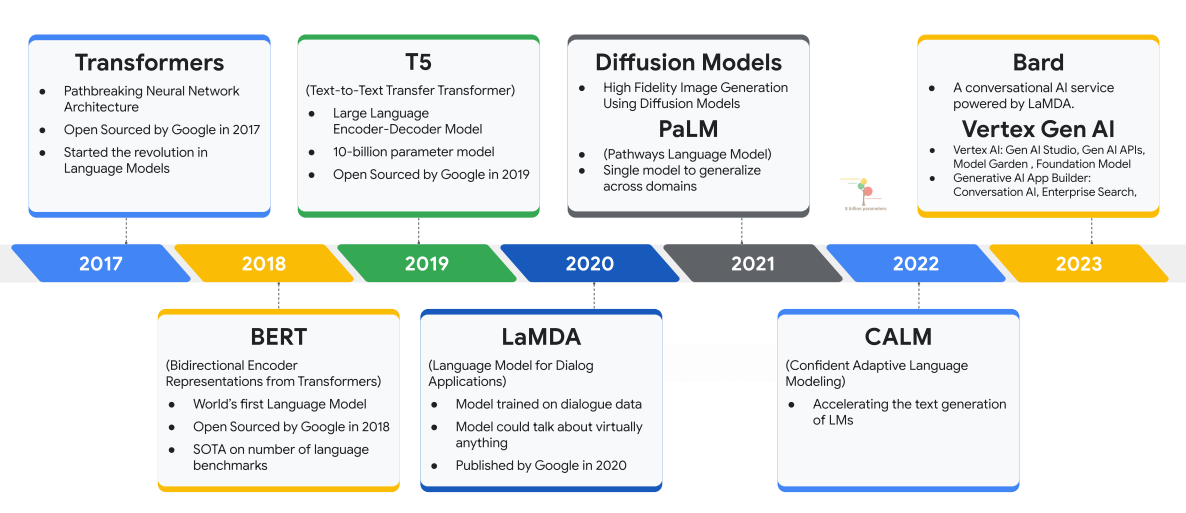
\includegraphics[width=\linewidth,keepaspectratio]{genai6}
\end{center}

{\tiny (Ref: Primer on LLM and Gen AI - Google Cloud)}
  
\end{frame}

%%%%%%%%%%%%%%%%%%%%%%%%%%%%%%%%%%%%%%%%%%%%%%%%%%%%%%%%%%%%%%%%%%%%%%%%%%%%%%%%%%
\begin{frame}[fragile]{Why are large language models different? }
\begin{columns}
    \begin{column}[T]{0.5\linewidth}
\begin{center}
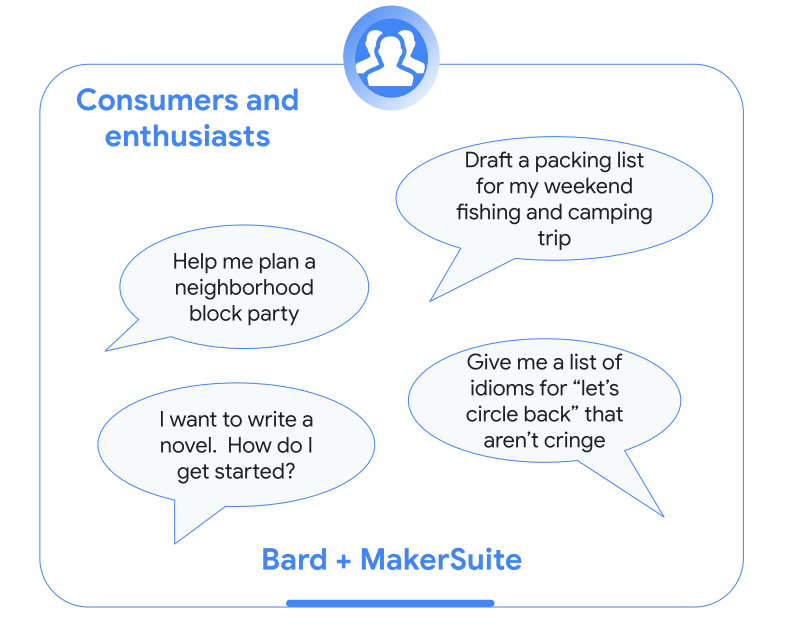
\includegraphics[width=\linewidth,keepaspectratio]{genai7}
\end{center}
    \end{column}
    \begin{column}[T]{0.5\linewidth}  
	
\begin{center}
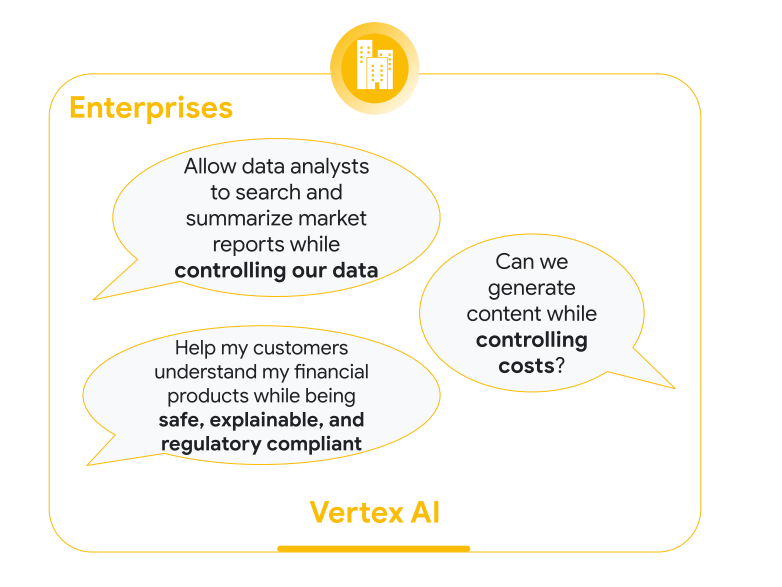
\includegraphics[width=\linewidth,keepaspectratio]{genai8}
\end{center}

    \end{column}
  \end{columns}
  
  
\end{frame}

%%%%%%%%%%%%%%%%%%%%%%%%%%%%%%%%%%%%%%%%%%%%%%%%%%%%%%%%%%%%%%%%%%%%%%%%%%%%%%%%%%
\section{Concepts}

%%%%%%%%%%%%%%%%%%%%%%%%%%%%%%%%%%%%%%%%%%%%%%%%%%%%%%%%%%%%%%%%%%%%%%%%%%%%%%%%%%
\begin{frame}[fragile]{Concepts}
\begin{itemize}
\item Generative AI trains algorithms to generate new data similar to existing data.
\item Google's generative AI tools use deep learning algorithms and neural networks.
\item Key concepts include autoencoders, GANs, and VAEs.
\end{itemize}
\end{frame}

%%%%%%%%%%%%%%%%%%%%%%%%%%%%%%%%%%%%%%%%%%%%%%%%%%%%%%%%%%%%%%%%%%%%%%%%%%%%%%%%%%
\begin{frame}[fragile]{What are large language models?}
\begin{columns}
    \begin{column}[T]{0.6\linewidth}
  \begin{itemize}
    \item ML algorithms that can recognize, predict, and generate human languages
    \item Pre-trained on petabyte scale text-based datasets resulting in large models with 10s to 100s of billions of parameters 
    \item LLMs are normally pre-trained on a large corpus of text followed by fi ne-tuning on a specifi c task
    \item LLMs can also be called Large Models (includes all types of data modality) and Generative AI (a model that produces content)
  \end{itemize}
    \end{column}
    \begin{column}[T]{0.4\linewidth}  
\begin{center}
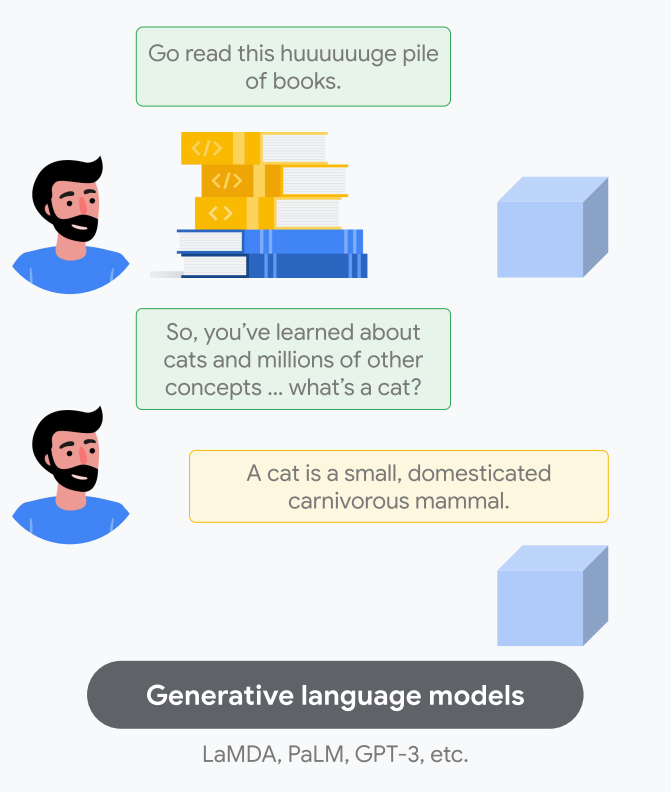
\includegraphics[width=0.8\linewidth,keepaspectratio]{genai4}
\end{center}
{\tiny (Ref: Primer on LLM and Gen AI - Google Cloud)}

    \end{column}
  \end{columns}
  
  
\end{frame}

%%%%%%%%%%%%%%%%%%%%%%%%%%%%%%%%%%%%%%%%%%%%%%%%%%%%%%%%%%%%%%%%%%%%%%%%%%%%%%%%%%
\begin{frame}[fragile]{Why are large language models different? }
\begin{columns}
    \begin{column}[T]{0.6\linewidth}
  \begin{itemize}
    \item LLMs are characterized by emergent abilities, or the ability to perform tasks that were not included in their training examples.
    \item LLMs contextual understanding of human language changes how we interact with data and intelligent systems.
	\item LLMs can find patterns and connections in massive, disparate data corpora.
  \end{itemize}
    \end{column}
    \begin{column}[T]{0.4\linewidth}  
\begin{center}
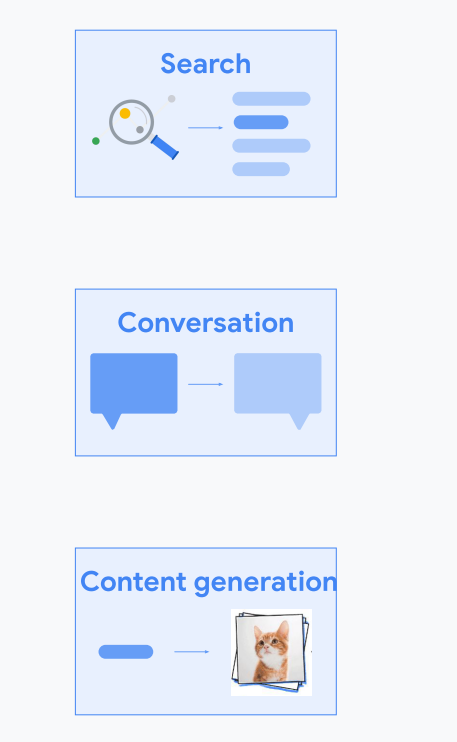
\includegraphics[width=0.5\linewidth,keepaspectratio]{genai5}
\end{center}
{\tiny (Ref: Primer on LLM and Gen AI - Google Cloud)}

    \end{column}
  \end{columns}
  
  
\end{frame}


%%%%%%%%%%%%%%%%%%%%%%%%%%%%%%%%%%%%%%%%%%%%%%%%%%%%%%%%%%%%%%%%%%%%%%%%%%%%%%%%%%
\section{Framework}

%%%%%%%%%%%%%%%%%%%%%%%%%%%%%%%%%%%%%%%%%%%%%%%%%%%%%%%%%%%%%%%%%%%%%%%%%%%%%%%%%%
\begin{frame}[fragile]{Framework}
\begin{itemize}
\item Google provides frameworks like TensorFlow, Keras, and PyTorch for generative AI development.
\item Pre-trained models and APIs like Cloud AutoML and Vertex AI are available.
\end{itemize}
\end{frame}

%%%%%%%%%%%%%%%%%%%%%%%%%%%%%%%%%%%%%%%%%%%%%%%%%%%%%%%%%%%%%%%%%%%%%%%%%%%%%%%%%%
\begin{frame}[fragile]{Vertex AI}

\begin{center}
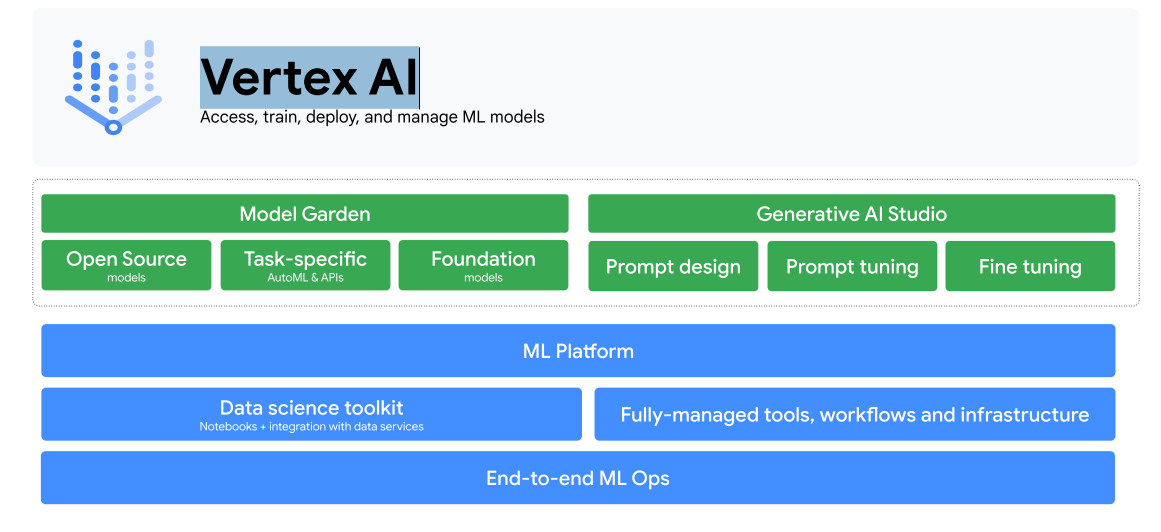
\includegraphics[width=\linewidth,keepaspectratio]{genai9}
\end{center}

{\tiny (Ref: Primer on LLM and Gen AI - Google Cloud)}
  
\end{frame}


%%%%%%%%%%%%%%%%%%%%%%%%%%%%%%%%%%%%%%%%%%%%%%%%%%%%%%%%%%%%%%%%%%%%%%%%%%%%%%%%%%
\section{Applications}

%%%%%%%%%%%%%%%%%%%%%%%%%%%%%%%%%%%%%%%%%%%%%%%%%%%%%%%%%%%%%%%%%%%%%%%%%%%%%%%%%%
\begin{frame}[fragile]{Applications}
\begin{itemize}
\item Generative AI applies to image/video generation, natural language processing, and music composition.
\item Google's tools are used in healthcare, finance, entertainment, and more.
\item Applications include Gmail, Docs, Slides, Sheets, and others.
\end{itemize}
\end{frame}

%%%%%%%%%%%%%%%%%%%%%%%%%%%%%%%%%%%%%%%%%%%%%%%%%%%%%%%%%%%%%%%%%%%%%%%%%%%%%%%%%%
\section{Conclusion}

%%%%%%%%%%%%%%%%%%%%%%%%%%%%%%%%%%%%%%%%%%%%%%%%%%%%%%%%%%%%%%%%%%%%%%%%%%%%%%%%%%
\begin{frame}[fragile]{Conclusion}
\begin{itemize}
\item Google's generative AI is a powerful technology with potential industry revolution.
\item Google leads with frameworks, tools, and pre-trained models.
\item Expect more innovative applications as the technology advances.
\end{itemize}
\end{frame}

%%%%%%%%%%%%%%%%%%%%%%%%%%%%%%%%%%%%%%%%%%%%%%%%%%%%%%%%%%%%%%%%%%%%%%%%%%%%%%%%%%
\begin{frame}[fragile]{References}

\begin{center}
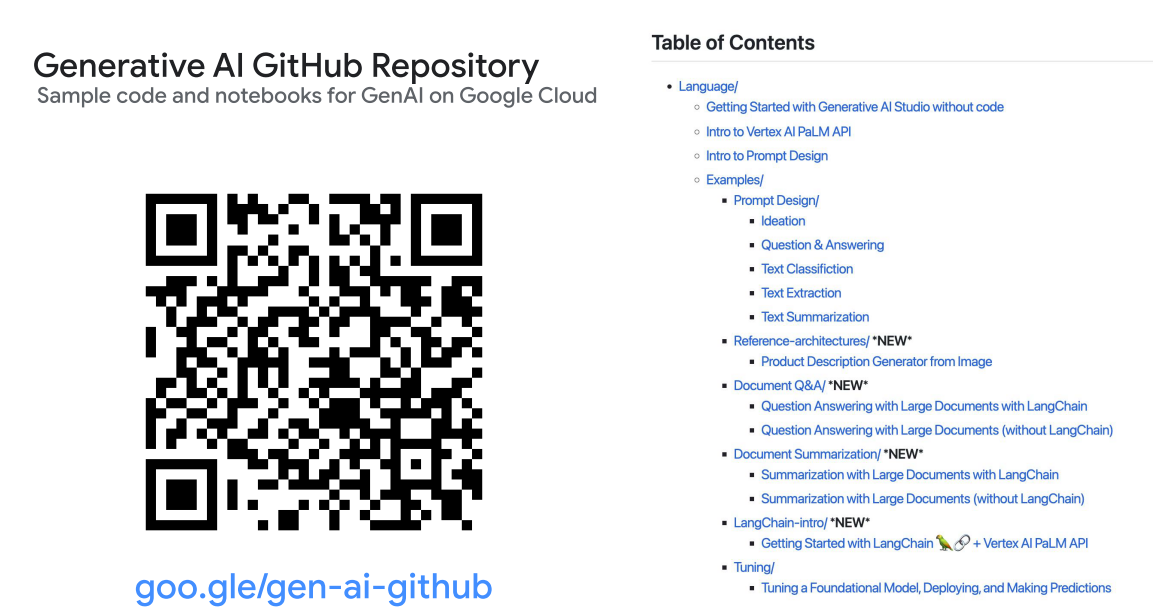
\includegraphics[width=\linewidth,keepaspectratio]{genai10}
\end{center}

{\tiny (Ref: Primer on LLM and Gen AI - Google Cloud)}
  
\end{frame}